\documentclass[12pt]{article}

\setlength\parindent{0pt}
\newcommand{\myt}[1]{\textbf{\underline{#1}}}

\usepackage{mathtools}
\usepackage{amssymb}
\usepackage{tikz,ifthen,amsmath,amssymb,fancyhdr,comment,lastpage}

\title{\vspace{-15ex}CS 241 Lecture 13\vspace{-1ex}}
\date{June 17th, 2015}
\author{Graham Cooper}

\begin{document}
	\maketitle
	
	Recall:\\
	$S \rightarrow$ S OP S $|$ a $|$ b $|$ c \\
	OP $\rightarrow +|-|*|/$\\
	
	Leftmost, rightmost derivation\\
	
	Derivations can be expressed naturally and succinctly as a tree structure\\
	
	For every leftmost (or rightmost) derivation, there is a unique parse tree.\\
	
	Example: Leftmost derivation for a+b*c\\
	
	$S \implies$ S Op S $\implies$ a Op S $\implies$ a + S $\implies$ a + S Op S \\
	$\implies$ a + b Op S $\implies$ a + b * S $\implies$ a + b * c\\
	
	OR\\
	
	$S \implies$ S Op S $\implies$ S Op S Op S $\implies$ a Op S Op S $\implies$ a + S Op S\\
	$\implies$ a + b Op S $\implies$ a + b * S $\implies$ a + b * c\\
	
	These correspond to different parse trees!\\
	
	\begin{center}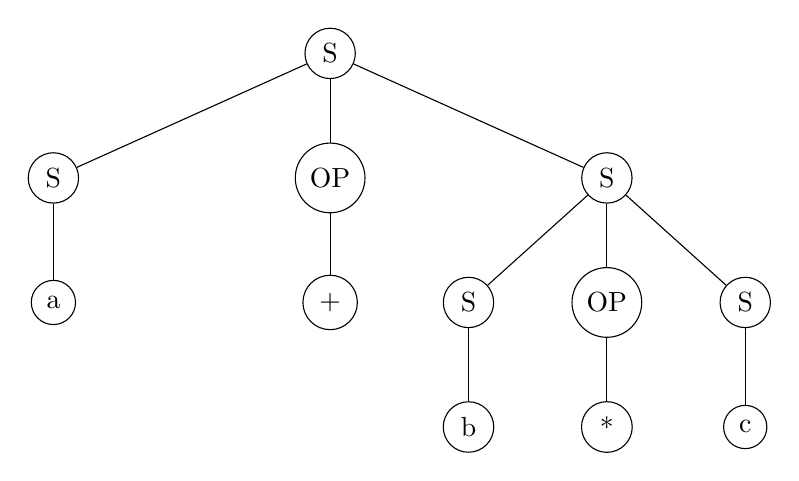
\begin{tikzpicture}[
		level distance=45 pt,
		every node/.style={circle,draw},
		level 1/.style={sibling distance=100 pt},
		level 2/.style={sibling distance=50 pt},
		level 3/.style={sibling distance=30 pt}
		]
		\node {S}
		child {node {S}
			child {node {a}}
		}
		child {node {OP}
			child {node {+}}
		}
		child {node {S}
			child {node {S}
				child {node {b}}
			}
			child {node {OP}
				child {node {*}}
			}
			child {node {S}
				child {node {c}}
			}
		}
		;
		\end{tikzpicture}\end{center}
	\begin{center}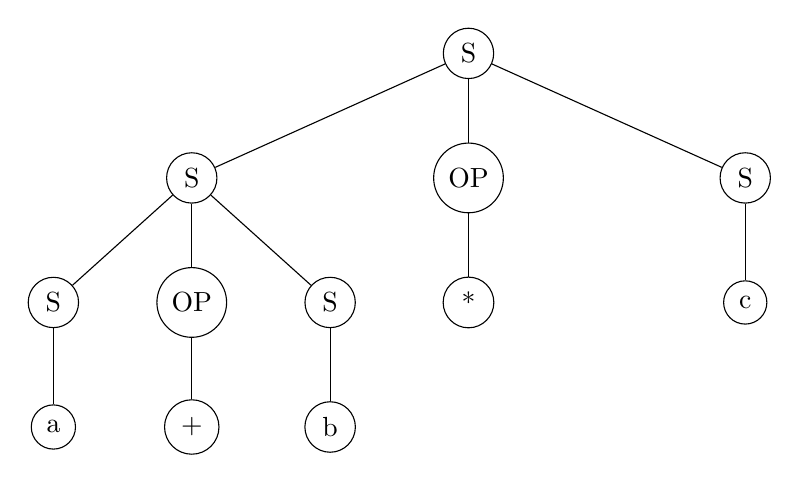
\begin{tikzpicture}[
		level distance=45 pt,
		every node/.style={circle,draw},
		level 1/.style={sibling distance=100 pt},
		level 2/.style={sibling distance=50 pt},
		level 3/.style={sibling distance=30 pt}
		]
		\node {S}
		child {node {S}
			child {node {S}
				child {node {a}}
			}
			child {node {OP}
				child {node {+}}
			}
			child {node {S}
				child {node {b}}
			}
		}
		child {node {OP}
			child {node {*}}
		}
		child {node {S}
			child {node {c}}
		}
		;
		\end{tikzpicture}\end{center}
	
	A grammar for whihc some word has more than one distinct leftmost derivation (equiv. $>$ 1 distinct parse tree) is called ambiguous.\\
	$S \implies S Op S | a | b | c$\\
	$Op \rightarrow + | - | * | /$\\
	(The above is an ambiguous grammar)\\
	If we only care whether w $\in$ L(G), ambiguity does not matter\\
	
	But as compiler writers, we want to know why w $\in$ L(G), ie, the derivation (or parse tree) matters\\
	
	\myt{WHY?} The shape of the parse tree describes the meaning of the string with respect to the grammar.\\
	
	So a word with $>$ 1 parse tree may have $>$ 1 meaning.\\
	
	The first tree above means that a + (b * c), but the second one is suggesting we are doing the plus first (a+b)*c\\
	
	So a + b * c could mean (a + b) * c or a + (b*c)\\
	
	\myt{What do we do?}\\
	
	\begin{enumerate}
		\item Use heuristics ("precedence") to guide the derivation process
		\item Make the grammar unambiguous\\
	\end{enumerate}
	
	$E \rightarrow$ E OP T | T\\
	$T \rightarrow$ a $|$ b $|$ c\\
	$OP \rightarrow$ + $|$ - $|$ * $|$ /\\
	
	a + b * c:\\
	E $\implies$ E OP T $\implies$ E OP T OP T $\implies$ T OP T OP T $\implies$\\
	 a OP T OP T $\implies$ a + T OP T $\implies$ a + b OP T \\
	 $\implies$ a + b * T $\implies$ a + b * c \\ 
	 
	 \begin{center}\begin{tikzpicture}[
	 	level distance=45 pt,
	 	every node/.style={circle,draw},
	 	level 1/.style={sibling distance=100 pt},
	 	level 2/.style={sibling distance=50 pt},
	 	level 3/.style={sibling distance=30 pt}
	 	]
	 	\node {E}
	 	child {node {E}
	 		child {node {E}
	 			child {node {T}
	 				child{node {a}}
	 			}
	 		}
	 		child {node {OP}
	 			child {node {+}}
	 		}
	 		child {node {T}
	 			child {node {b}}
	 		}
	 	}
	 	child {node {OP}
	 		child {node {*}}
	 	}
	 	child {node {T}
	 		child {node {c}}
	 	}
	 	;
	 	\end{tikzpicture}\end{center}
	 
	 Strict left-to-right precendence.\\
	 
	 What if we want to give *, / precedence over +, - ?\\
	 E $\rightarrow$ E PM T $|$ T\\
	 PM $\rightarrow$ + $|$ -\\
	 T $\rightarrow$ T TD F $|$ F \\
	 TD $\rightarrow$ * $|$ /\\
	 This way we have plus and minus on the left and product/division on the right.
	 
	 a + b * c\\
	 E $\implies$ E PM T $\implies$ T PM T $\implies$ F PM T $\implies$\\
	 a PM T $\implies$ a + T $\implies$ a + T TD F $\implies$ a + F TD F\\
	 $\implies$ a + b TD F $\implies$ a + b * F $\implies$ a + b * c\\
	 
	 \begin{center}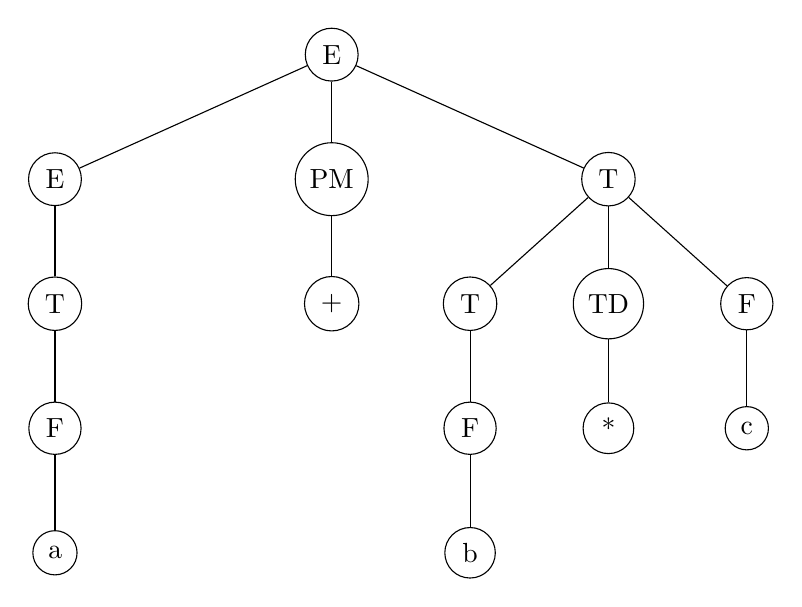
\begin{tikzpicture}[
	 	level distance=45 pt,
	 	every node/.style={circle,draw},
	 	level 1/.style={sibling distance=100 pt},
	 	level 2/.style={sibling distance=50 pt},
	 	level 3/.style={sibling distance=30 pt}
	 	]
	 	\node {E}
	 	child {node {E}
	 		child {node {T}
	 			child {node {F}
	 				child{node {a}}
	 			}
	 		}
	 	}
	 	child {node {PM}
	 		child {node {+}}
	 	}
	 	child {node {T}
	 		child {node {T}
	 			child {node {F}
	 				child {node {b}}
	 			}
	 		}
	 		child {node {TD}
	 			child {node {*}}
	 		}
	 		child {node {F}
	 			child {node {c}}
	 		}
	 	}
	 	;
	 	\end{tikzpicture}\end{center}
	 
	 We were successful in making the b * c have precedence\\
	 
	 \myt{Question:} If L is context-free, is there always an unambiguous grammar G such that L = L(G)?\\
	 
	 \myt{Answer:} NO! There are \underline{Inherently ambiguous languages} that only have ambiguous grammars\\
	 
	 \myt{Question:} Can we construct a tool that will tell whether a grammar is unambiguous.\\
	 
	 \myt{ANSWER:} NO! Undecidable\\
	 
	 Equivalence of grammars $G_1$, $G_2$, ie: $L(G_1) =? L(G_2)$ is also undecidable\\
	 
	 \section*{Recognizers}
	 
	 Recognizers - what class of computer programs is needed to recognize a CFL?\\
	 
	 - Regular Languages: DFA - essentially a program with finite memory\\
	 
	 - Context-free languages - NFA + stack - infinite memory, but its use is limited to LIFO order\\
	 
	 But we need more than just a yes/no answer!!\\
	 - Need the derivation (parse-tree) or an informative error message\\
	 
	 Problem of finding the derivation is called \underline{parsing}.\\
	 \underline{Given} Grammar G, start symbol S, terminal string w,\\
	 \underline{Find:} S$\implies$ ... $\implies$ w \\
	 - or report that there is no derivation\\
	 
	 How can we do this?\\
	 
	 2 Choices:\\
	 \begin{enumerate}
	 	\item Forwards - "top down parsing"\\
		 	start at S, expand non-terminals until you produce w
	 	\item Backwards - "bottom up parsing"\\
		 	Start at w, apply rules in reverse, produce S
	 \end{enumerate}
	 
	 Both options seem hard...\\
	 
	 \section*{Top-Down Parsing}
	 
	 Start at S, apply grammar rules, produce w\\
	 
	 S $\implies \alpha_1 \implies \alpha_2 \implies ... \implies$ w\\
	 
	 Use the stack to store intermediate steps $\alpha_i$ in reverse and match against characters in w.\\
	 
	 \underline{Invariant}: consumed input + reverse(stack contents) = $\alpha_i$ for some i\\
	
	
\end{document}
